\thaichapter{บทที่ 6}{การทดสอบและผลการดำเนินงาน}\addcontentsline{toc}{chapter}{บทที่ 6 การทดสอบและผลการดำเนินงาน}

ทุกข้อกำหนดของโจทย์ผ่านการทดสอบ ตารางต่อไปนี้สรุปวิธีทดสอบและผลที่ได้ ภาพหน้าจอประกอบอยู่ในภาคผนวก ขค.

\section*{6.1 ผลการทดสอบตามข้อกำหนด}\addcontentsline{toc}{section}{6.1 ผลการทดสอบตามข้อกำหนด}

\needspace{7\baselineskip}\noindent\textbf{ตารางที่ 6.1} ผลการทดสอบ

\begingroup\small\begin{longtable}[]{@{}>{\raggedright\arraybackslash}p{0.145\linewidth - 2\tabcolsep}>{\raggedright\arraybackslash}p{0.194\linewidth - 2\tabcolsep}>{\raggedright\arraybackslash}p{0.315\linewidth - 2\tabcolsep}>{\raggedright\arraybackslash}p{0.315\linewidth - 2\tabcolsep}@{}}
\toprule\noalign{}
ขั้น & สิ่งที่ทดสอบ & วิธีทดสอบ & ผล \\
\midrule\noalign{}
\endhead
\bottomrule\noalign{}
\endlastfoot
1 & เข้าเว็บด้วย HTTPS & เปิด \url{https://elephotelephus.site} และดูใบรับรองในเบราว์เซอร์ & ผ่าน ใบรับรองจาก Let's Encrypt และ http:// ถูกส่งต่อไป https:// \\
1 & ปิด root login & ssh root@เซิร์ฟเวอร์ & ผ่าน ได้ Permission denied \\
1 & ปิดรหัสผ่าน ใช้กุญแจเท่านั้น & sudo sshd -T กรอง permitrootlogin, passwordauthentication, authenticationmethods & ผ่าน ค่าเป็น no, no, publickey \\
1 & เวอร์ชันซอฟต์แวร์ & ดูไฟล์ versions.txt ที่ setup.sh สร้าง & ได้เวอร์ชันตามตารางที่ 3.1 \\
1 & fail2ban ทำงาน & sudo fail2ban-client status & ผ่าน มี 3 jail: sshd, wordpress-login, nginx-limit-req \\
2 & บล็อกต่างประเทศ & ทดสอบจากเครื่องต่างประเทศหลายจุดด้วย check-host.net & ผ่าน เครื่องต่างประเทศหมดเวลา (timeout) ทั้งหมด \\
2 & เข้าได้จากไทย & เปิดเว็บและ SSH จากเน็ตบ้าน หอพัก และมือถือในไทย & ผ่าน \\
2 & บันทึกการบล็อก & sudo geo-firewall.sh status และ log GEO-BLOCK & ผ่าน มีช่วง IP ไทย 1,167 ช่วง และมี log ของ IP ต่างประเทศ \\
3 & เว็บไซต์บนมือถือและคอมพิวเตอร์ & เปิดทุกหน้าบนหน้าจอหลายขนาด & ผ่าน \\
3 & นำเข้าข่าวคณะ & สั่งนำเข้าแล้วตรวจตาราง wp\_posts ด้วย DBeaver & ผ่าน ข่าวถูกบันทึกพร้อมลิงก์ต้นทาง และไม่ซ้ำ \\
เพิ่มเติม & ฐานข้อมูลไม่เปิดสู่ภายนอก & sudo ss -ltnp กรอง 3306 & ผ่าน ฟังเฉพาะ 127.0.0.1:3306 \\
เพิ่มเติม & dashboard และ AI & รัน secdash-collect.py แล้วเปิดหน้า ความปลอดภัย & ผ่าน แสดงข้อมูลจริงและสรุปภาษาไทยจาก Gemini \\
\end{longtable}\endgroup

\begin{figure}[!htbp]
\centering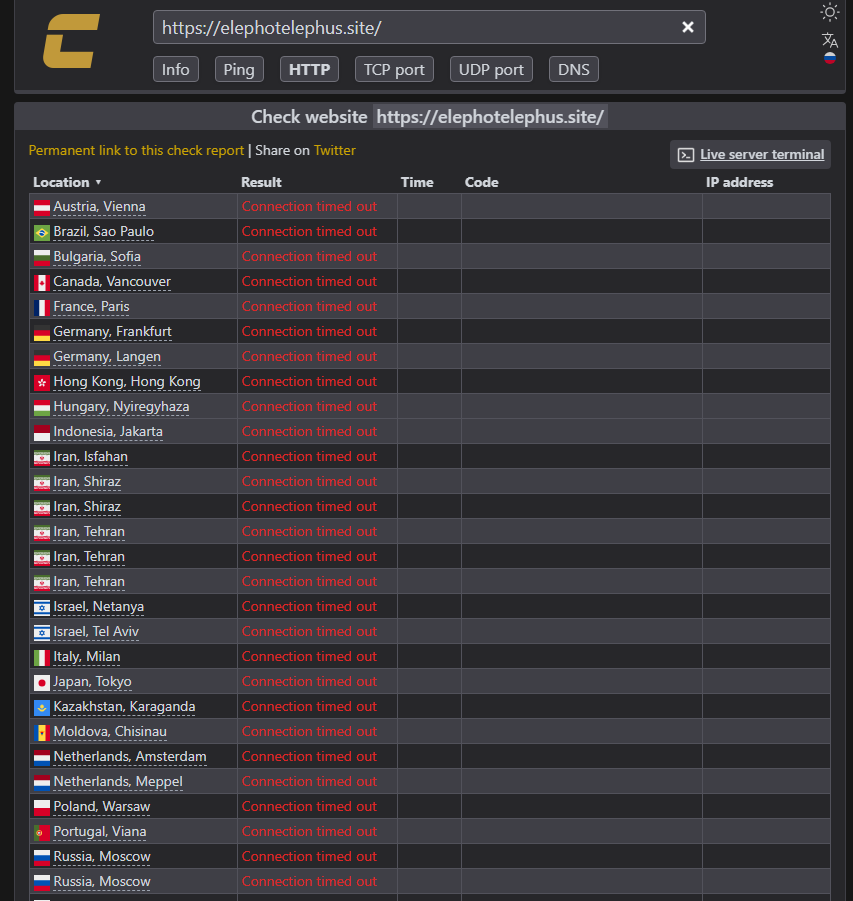
\includegraphics[width=0.78\linewidth,height=0.42\textheight,keepaspectratio]{figures/check-host.png}
\caption*{\textbf{ภาพที่ 6.1} ทดสอบเข้าเว็บไซต์จากเครื่องในหลายประเทศด้วย check-host.net ทุกจุดหมดเวลา (Connection timed out)}
\end{figure}

\begin{figure}[!htbp]
\centering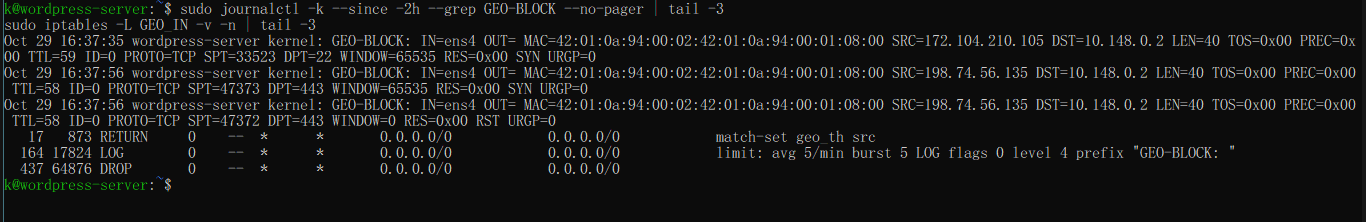
\includegraphics[width=1.00\linewidth,height=0.42\textheight,keepaspectratio]{figures/geo-block-log.png}
\caption*{\textbf{ภาพที่ 6.2} log GEO-BLOCK ของ IP ต่างประเทศที่พยายามต่อพอร์ต 22 และ 443 และตัวนับของ chain GEO\_IN}
\end{figure}

\section*{6.2 การโจมตีที่ตรวจพบจริง}\addcontentsline{toc}{section}{6.2 การโจมตีที่ตรวจพบจริง}

ข้อมูลจาก dashboard เมื่อวันที่ 29 ตุลาคม 2569 ทุกตัวเลขมาจาก log จริงของเซิร์ฟเวอร์ ไม่มีข้อมูลจำลอง

\begin{figure}[!htbp]
\centering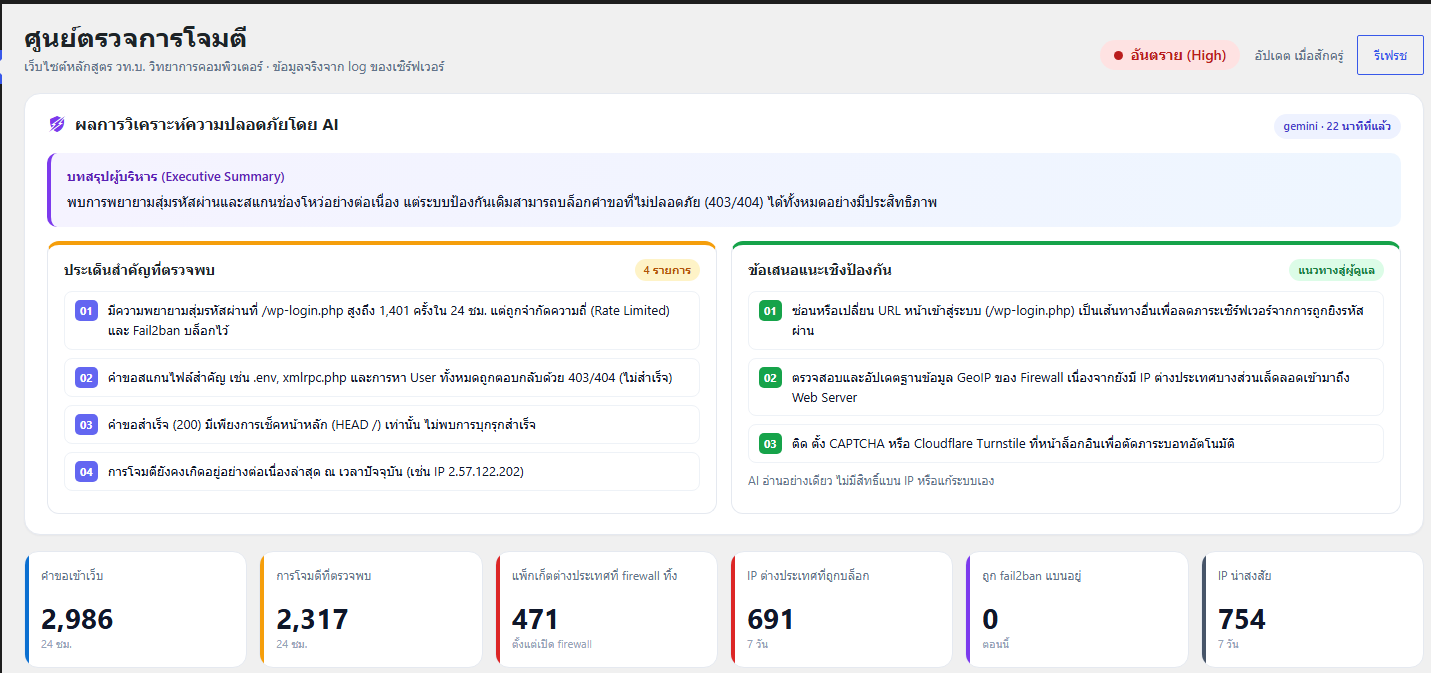
\includegraphics[width=1.00\linewidth,height=0.42\textheight,keepaspectratio]{figures/dashboard-ai.png}
\caption*{\textbf{ภาพที่ 6.3} กล่องสรุปจาก AI (Gemini) และตัวเลขหลักของ dashboard}
\end{figure}

\begingroup\small\begin{longtable}[]{@{}>{\raggedright\arraybackslash}p{0.485\linewidth - 2\tabcolsep}>{\raggedright\arraybackslash}p{0.485\linewidth - 2\tabcolsep}@{}}
\toprule\noalign{}
ตัวชี้วัด & ค่า \\
\midrule\noalign{}
\endhead
\bottomrule\noalign{}
\endlastfoot
คำขอเข้าเว็บ (24 ชม.) & 2,986 ครั้ง \\
การโจมตีที่ตรวจพบ (24 ชม.) & 2,317 เหตุการณ์ \\
SSH เข้าไม่สำเร็จ (24 ชม.) & 212 ครั้ง (ไม่มีครั้งใดสำเร็จ เพราะใช้กุญแจเท่านั้น) \\
/wp-login.php ถูกโจมตี (7 วัน) & 2,734 ครั้ง \\
IP ต่างประเทศที่ถูกบล็อก (7 วัน) & 691 IP \\
แพ็กเก็ตต่างประเทศที่ firewall ทิ้ง (ตั้งแต่เปิดใหม่) & 471 แพ็กเก็ต \\
ผลลัพธ์ HTTP (24 ชม.) & 2xx 2,280 · 3xx 130 · 4xx 577 · 5xx 0 \\
\end{longtable}\endgroup

\begin{figure}[!htbp]
\centering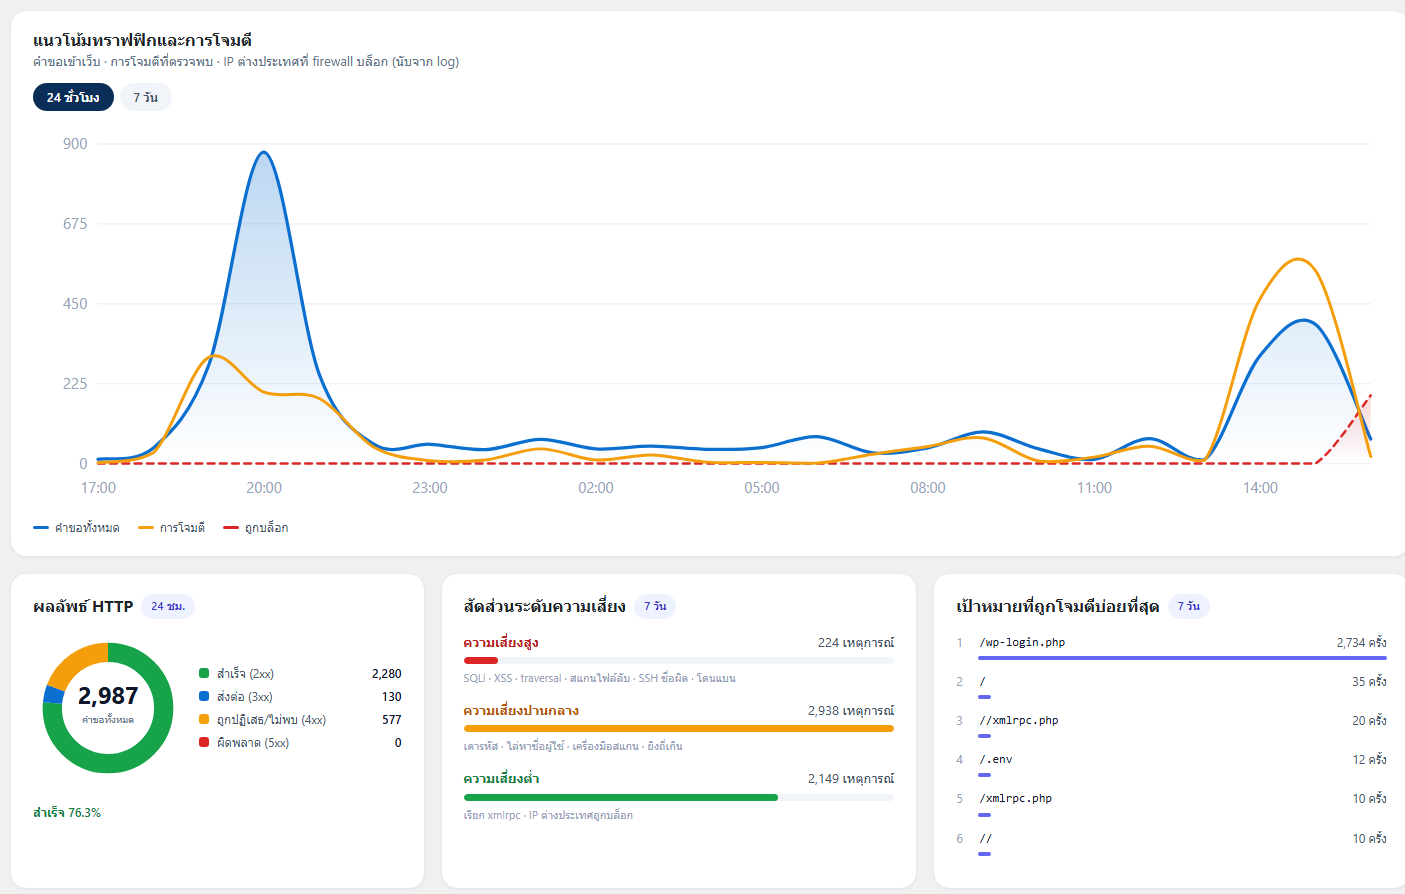
\includegraphics[width=1.00\linewidth,height=0.42\textheight,keepaspectratio]{figures/dashboard-chart.png}
\caption*{\textbf{ภาพที่ 6.4} กราฟ 24 ชั่วโมง สัดส่วนผลลัพธ์ HTTP ระดับความเสี่ยง และ URL ที่ถูกโจมตีบ่อยที่สุด}
\end{figure}

สิ่งที่พบ

\begin{itemize}
\tightlist
\item
  การโจมตีส่วนใหญ่เป็นการเดารหัสผ่านที่ /wp-login.php IP อันดับหนึ่งคือ 64.227.79.185 (ต่างประเทศ) 1,004 เหตุการณ์ ทุกครั้งถูก rate limit (429) และไม่มีครั้งใดเข้าระบบได้
\item
  IP 92.118.39.77 พยายามเข้า SSH ด้วยชื่อผู้ใช้ที่ไม่มีอยู่ และถูก fail2ban แบนอัตโนมัติ
\item
  คำขอไฟล์ลับ (.env) และ xmlrpc.php ถูกปฏิเสธทุกครั้ง
\item
  ไม่มีข้อผิดพลาด 5xx เลย เซิร์ฟเวอร์ให้บริการได้ปกติแม้ถูกโจมตีต่อเนื่อง
\end{itemize}

\begin{figure}[!htbp]
\centering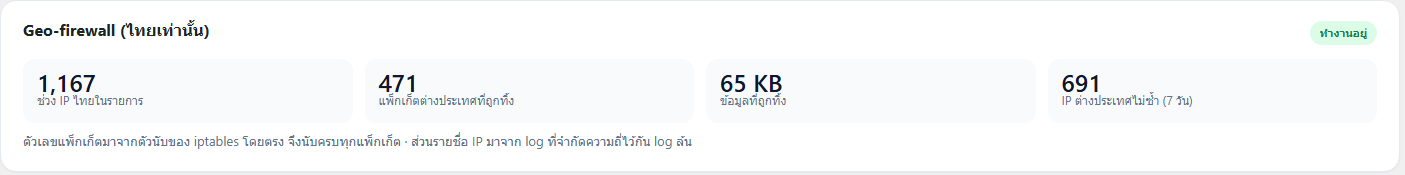
\includegraphics[width=1.00\linewidth,height=0.42\textheight,keepaspectratio]{figures/dashboard-firewall.png}
\caption*{\textbf{ภาพที่ 6.5} การ์ด Geo-firewall: ช่วง IP ไทย 1,167 ช่วง และตัวนับแพ็กเก็ตที่ถูกทิ้งจาก iptables}
\end{figure}

\begin{figure}[!htbp]
\centering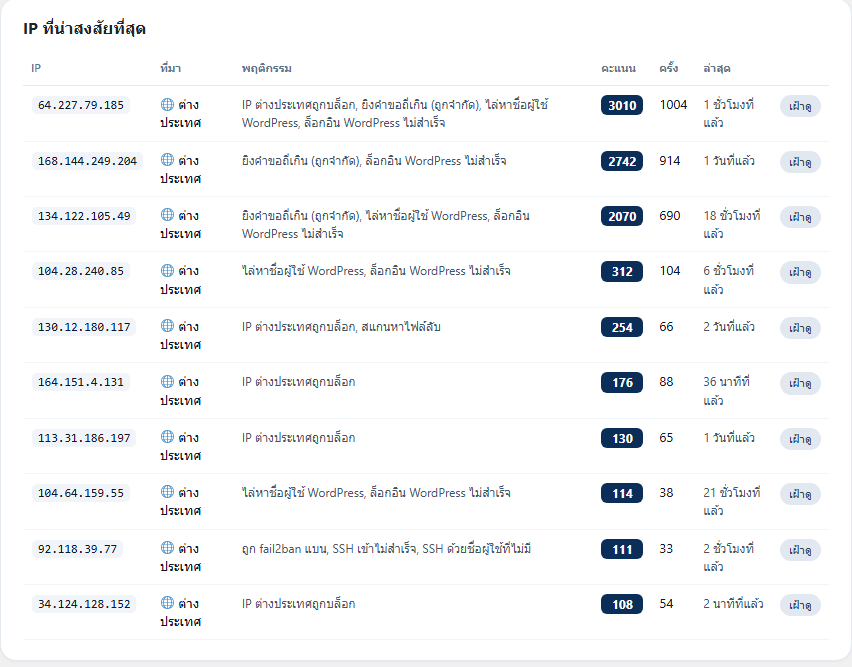
\includegraphics[width=0.77\linewidth,height=0.42\textheight,keepaspectratio]{figures/dashboard-top-ip.png}
\caption*{\textbf{ภาพที่ 6.6} IP ที่น่าสงสัยที่สุด จัดอันดับตามคะแนนความเสี่ยง}
\end{figure}

ข้อสังเกตสำคัญ: ช่วงวันที่ 28--29 ตุลาคม geo-firewall ปิดอยู่ชั่วคราว เพราะผู้ดูแลสั่ง apply ใหม่แต่ไม่ได้ยืนยันภายใน 3 นาที ระบบจึงย้อนกลับเองตามที่ออกแบบไว้ ในช่วงนั้นกราฟแสดงคำขอและการโจมตีพุ่งสูงทันที (ช่วง 20:00 และ 14:00--16:00) เมื่อเปิด firewall กลับมา เส้น ``ถูกบล็อก'' จึงเพิ่มขึ้นแทน เหตุการณ์นี้แสดงให้เห็นทั้งความสำคัญของ firewall และประโยชน์ของการป้องกันหลายชั้น เพราะระหว่างที่ firewall ปิด rate limit, fail2ban และ SSH แบบกุญแจยังกันการบุกรุกไว้ได้ทั้งหมด

นอกจากนี้ในตาราง IP พบ 34.124.128.152 ซึ่งเป็น IP ของเซิร์ฟเวอร์เอง ถูกนับเป็น IP ต่างประเทศ เกิดจาก WordPress เรียกตัวเองผ่านโดเมน (WP-Cron) แล้วถูก geo-firewall บล็อก คณะผู้จัดทำแก้โดยให้ geo-firewall อนุญาต IP ของเซิร์ฟเวอร์เองโดยอัตโนมัติ (ดูบทที่ 7)

\section*{6.3 การตรวจสอบคำแนะนำของ AI}\addcontentsline{toc}{section}{6.3 การตรวจสอบคำแนะนำของ AI}

AI สรุปว่า ``พบการสแกนหาไฟล์ตั้งค่าความลับตระกูล .env และการค้นหาชื่อผู้ใช้ WordPress จาก IP ต่างประเทศอย่างต่อเนื่อง'' คณะผู้จัดทำนำคำแนะนำมาตรวจกับระบบจริงก่อนนำไปใช้

\begingroup\small\begin{longtable}[]{@{}>{\raggedright\arraybackslash}p{0.425\linewidth - 2\tabcolsep}>{\raggedright\arraybackslash}p{0.545\linewidth - 2\tabcolsep}@{}}
\toprule\noalign{}
คำแนะนำของ AI & ผลการตรวจ \\
\midrule\noalign{}
\endhead
\bottomrule\noalign{}
\endlastfoot
ตั้งค่าเว็บเซิร์ฟเวอร์ให้ปฏิเสธไฟล์ .env & ทำไว้แล้วตั้งแต่ติดตั้ง (location \textasciitilde{} /.) \\
บล็อก IP ที่สแกน และพิจารณา GeoIP blocking & มี geo-firewall และ fail2ban อยู่แล้ว คำแนะนำนี้เกิดจาก AI ไม่ทราบบริบท \\
ปิดการไล่หาชื่อผู้ใช้และจำกัด REST API & ถูกต้อง ยังไม่ได้ปิด เป็นงานที่ควรทำต่อ (บทที่ 7) \\
\end{longtable}\endgroup

คณะผู้จัดทำจึงปรับให้สคริปต์ส่งรายการมาตรการที่มีอยู่ และ status code ของแต่ละคำขอให้ AI ด้วย ผลคือ AI ต้องใช้ควบคู่กับการตัดสินใจของคน ไม่ควรเชื่อตามทุกข้อ
